\documentclass{llncs}

%\usepackage{showframe}
\usepackage[utf8]{inputenc}
\usepackage{times}
\usepackage{url}
\usepackage{latexsym}
\usepackage{color}
\usepackage{tikz}
\usepackage{pgfplots}
\usepackage{lipsum}
\usepackage{units}
\usepackage{amsmath}
\usepackage{amssymb}
\usepackage{relsize}
\usepackage{booktabs}
\usepackage{multirow}
\usepackage{subfigure}
\usepackage[inline]{enumitem}
\usepackage{varwidth}
\usepackage{mathabx}
\usepackage[square,numbers,sectionbib]{natbib}
\usepackage{marginnote}

\usetikzlibrary{arrows, backgrounds, decorations.markings, positioning, shapes}

\renewcommand\bibnumfmt[1]{#1.}

\newcommand\newcite[2][]{\ifthenelse{\equal{#1}{}}{\citet{#2}}{\citet[#1]{#2}}}

\newcommand\TODO[1]{\textcolor{red}{[TODO #1]}}
\newcommand\REVIEW[1]{}%\textcolor{green}{[REVIEW \textit{``#1''}]}}
\newcommand\REVIEWOK[1]{}%\marginnote{\textcolor{green}{\underline{Reviewer said:} \textit{``#1''}}}}
\newcommand\ANNOTATE[2]{\textcolor{blue}{[#1 \textbf{$\rightarrow$ #2}]}}
\newcommand\FILL[1]{\textcolor{red}{\lipsum[#1]}}

\title{Graph Co-Ranking Approach to Keyphrase Annotation\\for Digital Libraries}

\author{
%  Adrien Bougouin\thanks{
%    The authors would like to thank the anonymous reviewers for their useful
%    advice and comments. This work was supported by the French National Research
%    Agency (TermITH project -- ANR-12-CORD-0029).
%  } \and Florian Boudin \and Béatrice Daille
}
\institute{
%  Université de Nantes, LINA, France
}

\begin{document}
  \maketitle

  \begin{abstract}
    % abstract similar to http://www.dcs.gla.ac.uk/~zhouke/papers/ecir2015-zhou.pdf
    Keyphrase annotation is the task of identifying textual units that represent the main content of a document.
    Automatic keyphrase annotation methods fall into two disjoint categories: extraction, which outputs keyphrases directly from the textual units within the content of the document; and assignment, which identifies keyphra\-ses controlled by domain-specific vocabularies.
    Many keyphrase extraction methods have been proposed, whereas keyphrase assignment methods have rarely been proposed. %because of assignment difficulty compared to extraction.
    However, keyphrase-based document indexing for Digital Libraries requires both categories of methods.
    % abstract similar to http://frncsrss.github.io/papers/rousseau-ecir2015.pdf
    In this paper, we apply the concept of co-ranking for simultaneously extracting and assigning keyphrases from a graph combining document topics and domain-specific keyphrases.
    This approach leverages the global context --- the domain --- of the document to better extract key\-phrases from the topics, and the local context --- the document --- of domain-specific keyphrases to better assign keyphrases that cannot be extracted from the document.
    To the best of our knowledge, this is the first attempt to simultaneously perform both keyphrase extraction and assignment.
    Experiments on three evaluation datasets show statistically significant improvements in f1-score compared to state-of-the-art results.

%    Keyphrases are words or phrases that summarize the content of a document.
%    In previous work, automatic keyphrase annotation is either carried out 
%    by extracting the most important phrases from a document (keyphrase 
%    extraction), or by assigning entries from controlled vocabulary 
%   (keyphrase assignment).
%    On the one hand, assignment methods provide better-formed keyphrases, 
%   as well as keyphrases that do not occur in the document.
%    On the other hand, extraction methods do not depend on manually built 
%    resources and are able to provide new (not already assigned) keyphrases.
%    This paper proposes a new method that uses graph co-ranking to perform both
%    keyphrase extraction and keyphrase assignment, in a mutual reinforcing manner.
%    Experimental results show the effectiveness of the proposed method, which
%    outperforms both keyphrase extraction and keyphrase assignment baselines.

    \keywords{
        Digital Libraries;
        keyphrase annotation;
        graph co-ranking;
        keyphrase extraction;
        keyphrase assignment.
    }
  \end{abstract}

  \section{Introduction}
\label{sec:section}
    Keyphrases are words or phrases that represent the main content of a document.
    Similar to an abstract, keyphrases give a synoptic picture of what is important in the document.
    Disimilar to an abstract, keyphrases are small grain units and are useful resources for many Natural Language Processing tasks: document clustering~\cite{han2007webdocumentclustering}, information retrieval~\cite{medelyan2008smalltrainingset}, document summarization~\cite{litvak2008graphbased}, etc.
    However, documents do not always contain keyphrases.
    As the daily flow of new documents grows, manually annotating documents has become impractical.
    Hence automatic keyphrase extraction recently attracts a lot of attention and many different methods are proposed~\cite{hasan2014state_of_the_art}.

    Automatic keyphrase extraction is the task of detecting important words or phrases within a document.
    Generally speaking, we divide keyphrase extraction methods into two categories: supervised and unsupervised.
    Supervised methods treat keyphrase extraction as a binary classification task, e.g.~\cite{witten1999kea}.
    Conversely, unsupervised methods usually rank keyphrase candidates by importance and select the top-ranked ones as keyphrases, e.g.~\cite{mihalcea2004textrank}.

    Although they tackle the keyphrase extraction problem differently, both supervised and unsupervised methods rely on a candidate selection step.
    Keyphrase candidate selection identifies words or phrases consistent with human-assigned keyphrase properties.
    %Although keyphrase candidate selection starts to draw attention~\cite{wang2014keyphraseextractionpreprocessing}, keyphrase extraction methods use simple heuristics: selection of n-grams, sequences of nouns and adjectives, etc.
    However, current selection methods use simple heuristics~\cite{wang2014keyphraseextractionpreprocessing}: candidates are n-grams or sequences of nouns and adjectives.
    %This work infers linguistic properties from human-assigned keyphrases and demonstrates their applicability on keyphrase candidate selection.
    This work proposes rules based on a comprehensive analysis of modifiers within human-assigned keyphrases.
    We demonstrate their applicability on keyphrase candidate selection.
    
    This paper is organized as follows.
    Section~\ref{sec:keyphrase_properties} presents an analysis of human-assigned keyphrases.
    Section~\ref{sec:candidate_selection} describes common keyphrase candidate selection methods followed by a description of our method in Section~\ref{sec:proposed_candidate_selection_method}. Finally, Section~\ref{sec:experiments} presents the expriments and Section~\ref{sec:conclusion} concludes our work.

  \section{Related Work}
\label{sec:related_work}
  \TODO{Introduction to the standard pipeline}

  \subsection{Automatic Keyphrase Extraction}
  \label{subsec:ake}
    \begin{itemize}
      \item{TF-IDF, Likey, etc.}
      \item{Graph-based methods (focus on TopicRank)}
      \item{GenEX, KEA, HUMB, etc. (focus on KEA)}
    \end{itemize}

  \subsection{Automatic Keyphrase Assignment}
  \label{subsec:aka}
    \begin{itemize}
      \item{KEA++ (Automatic Keyphrase Indexing)}
      \item{WAM (SMT AKA method)}
    \end{itemize}

  \subsection{Graph co-ranking for NLP}
  \label{subsec:graph_co_ranking_for_nlp}
    \begin{itemize}
      \item{Xiaojun Wan: Cross-language document summarization}
      \item{Rui Yan: Tweet recommendation}
      \item{Kang Liu: Opinion mining (check) from online reviews}
    \end{itemize}


  \begin{frame}{Contributions}\framesubtitle{TopicCoRank}
  \begin{alertblock}{TODO}
    \begin{itemize}
      \item{Extension supervisée de TopicRank}
      \item{Adaptaion en domaines de spécialité}
      \item{$\Rightarrow$ Assignement}
      \item{Problèmes identifiés de l'assignement}
    \end{itemize}
  \end{alertblock}
\end{frame}

\begin{frame}{TopicCoRank}\framesubtitle{Proposition}
\end{frame}

\begin{frame}{TopicCoRank}\framesubtitle{Exemple}
\end{frame}

\begin{frame}{TopicCoRank}\framesubtitle{Évaluation}
\end{frame}

\begin{frame}{TopicCoRank}\framesubtitle{Résultats}
\end{frame}

\begin{frame}{TopicCoRank}\framesubtitle{Bilan}
\end{frame}


  \section{Experimental Setup}
\label{sec:experimental_setup}
    \subsection{Datasets}
    \label{subsec:datasets}
    
        We conduct our experiments on data from the DEFT-2016 benchmark datasets~\cite{daille-et-al:2016:DEFT}\footnote{Data has been provided by the TermITH project for both DEFT-2016 and this work. Parallely, the subset division has been modified for the purpose of DEFT-2016. Therefore, we use the same data as DEFT-2016, but the subset division is different. The subset division we used for our experiences can be found here: \url{https://github.com/adrien-bougouin/KeyBench/tree/coling_2016/datasets/}} in three domains: linguistics, information Science and archaeology.
        %
        Table~\ref{tab:dataset_statistics} shows the factual information about the datasets.
        %
        Each dataset is a collection of 706 up to 718 French bibliographic records collected from the database of the French Institute for Scientific and Technical Information\footnote{\url{http://www.inist.fr}} (Inist).
        The bibliographic records contain a title of one scientific paper, its abstract and its keyphrases that were annotated by professional indexers (one per bibliographic record).
        Indexers were given the instruction to assign reference keyphrases from a controlled vocabulary and to extract new concepts or very specific keyphrases from the titles and the abstracts.
        %We divided each corpora into three sets: a test set, used for evaluation; a training set (denoted as train), used to represent the domain; and a development set (denoted as dev), used for parameter tuning.
        Each dataset is divided into three sets: a test set, used for evaluation; a training set (denoted as train), used to represent the domain; and a development set (denoted as dev), used for parameter tuning.
        %
        %The test set is composed of 200 bibliographic records, the train set is composed of the remaining and the development includes 100 of the bibliographic records from the training set.
        
            \begin{table}[htb!]
            \centering
            \begin{tabular}{l|c@{\hspace{1em}}c@{\hspace{1em}}c@{\hspace{.5em}}|@{\hspace{.5em}}c@{\hspace{1em}}c@{\hspace{1em}}c@{\hspace{.5em}}|@{\hspace{.5em}}c@{\hspace{1em}}c@{\hspace{1em}}c}
            \toprule
                \multirow{2}{*}{\textbf{Corpus}} & \multicolumn{3}{c@{\hspace{.5em}}|@{\hspace{.5em}}}{\textbf{Linguistics}} & \multicolumn{3}{c@{\hspace{.5em}}|@{\hspace{.5em}}}{\textbf{Information Science}} & \multicolumn{3}{c}{\textbf{Archaeology}}\\
                \cline{2-10}
                & \multicolumn{1}{c@{~$\supset$}}{train} & dev & test & \multicolumn{1}{c@{~$\supset$}}{train} & dev & test & \multicolumn{1}{c@{~$\supset$}}{train} & dev & test\\
                \hline
                Documents & 515 & 100 & 200  & 506 & 100 & 200 & 518 & 100 & 200\\
                Tokens/Document & 161 & 151 & 147 & 105 & 152 & 157 & 221 & 201 & 214\\
                Keyphrases & 8.6 & 8.8 & 8.9 & 7.8 & 10.0 & 10.2 & 16.9 & 16.4 & 15.6\\
                Missing Keyphrases (\%) & 60.6 & 63.2 & 62.8 & 67.9 & 63.1 & 66.9 & 37.0 & 48.4 & 37.4\\
                \bottomrule
            \end{tabular}
            \caption{
                Dataset statistics.
                ``Missing'' represents the percentage of keyphrases that cannot be retrieved within the documents.
                \label{tab:dataset_statistics}}
        \end{table}

        The amount of missing keyphrases, i.e.~keyphrases that cannot be extracted from the documents, shows the importance of keyphrase assignment in the context of scientific domains.
        More than half of the keyphrases of linguistics and information science domains can only be assigned, which confirms that these two datasets are difficult to process with keyword extraction approaches alone. 
        %Other non domain-specific and non scientific datasets used in the keyphrase extraction community contain much lower amounts of missing keyphrases, such as the DUC dataset~\cite{wan2008expandrank} that contains about 4\% of missing keyphrases.

    \subsection{Document preprocessing}
    \label{subsec:document_preprocessing}
        We apply the following preprocessing steps to each document: sentence segmentation, word tokenization and Part-of-Speech (POS) tagging.
        Sentence segmentation is performed with the PunktSentenceTokenizer provided by the Python Natural Language ToolKit (NLTK)~\cite{bird2009nltk}, word tokenization using the Bonsai word tokenizer\footnote{The Bonsai word tokenizer is a tool provided with the Bonsai PCFG-LA parser: \url{http://alpage.inria.fr/statgram/frdep/fr_stat_dep_parsing.html}} and POS tagging with MElt~\cite{denis2009melt}.

    \subsection{Baselines}
    \label{subsec:baselines}
        To show the effectiveness of our approach, we compare TopicCoRank and its variants (TopicCoRank$_\textnormal{\textit{extr}}$ and TopicCoRank$_\textnormal{\textit{assign}}$) with TopicRank and KEA++.
        For KEA++, we use the thesauri maintained by Inist\footnote{Thesauri are available from: \url{http://deft2016.univ-nantes.fr/download/traindev/}} to index the bibliographic records of Linguistics, Information Science and Archaeology.
    
    % \subsection{Evaluation measures}
    % \label{subsec:evaluation_measures}
    %     To evaluate the performance of the keyphrase extraction methods, we use the common measures of precision (P), recall (R) and f1-score (F).
    %     Following previous work~\cite{bougouin2013topicrank}, we cut off the extracted keyphrases at the ten best ranked ones and perform the comparisons with stemmed keyphrases.
    
    %     Consistent with \newcite{hassan2010conundrums}, we also report the performance of TopicCoRank and the baselines in terms of precision-recall curves.
    %     Such representation gives a good appreciation of the advantage of a method compared to others, especially if the other methods achieve performances in the \textit{Area Under the Curve} (AUC).
    %     To generate the curves, we vary the evaluation cut-off from 1 to the total number of extracted/assigned keyphrases and compute the precision and recall for each cut-off.

    \subsection{TopicCoRank setting}
    \label{subsec:topiccorank_settings}
        \REVIEWOK{Empirically, we'd tune the parameters on development set, which is independant of evaluation dataset}
        The $\lambda_t$ and $\lambda_k$ parameters of TopicCoRank were tuned on the development sets, and set to 0.1 and 0.5 respectively.
        %To achieve a near-optimal performance with TopicCoRank, we empirically tune $\lambda_t$ and $\lambda_k$ on the development sets.
        %For each dataset, the near-optimal value of $\lambda_t$ is 0.1 and the near-optimal value of $\lambda_k$ is 0.5.
        This empirical setup means that the importance of topics is much more influenced by controlled keyphrases than other topics, and that the importance of controlled keyphrases is equally influenced by controlled keyphrases and topics.
        In other words, the domain has a positive influence on the joint task of keyphrase extraction and assignment.
        % \begin{table}
        %     \centering
        %     \begin{tabular}{l|c|c|c|c|c|c|c|c|c}
        %         \toprule
        %         \multirow{2}{*}{$\lambda_k$} & \multicolumn{9}{c}{$\lambda_t$}\\
        %         \cline{2-10}
        %         & \textbf{0.10} & 0.20 & 0.30 & 0.40 & 0.50 & 0.60 & 0.70 & 0.80 & 0.90\\
        %         \hline
        %         0.10 & 0.265929 & 0.223061 & 0.220135 & 0.210187 & 0.205136 & 0.200050 & 0.182961 & 0.163289 & 0.152953\\
        %         \hline
        %         0.20 & 0.308469 & 0.268461 & 0.235401 & 0.220135 & 0.208541 & 0.200926 & 0.180708 & 0.163300 & 0.145991\\
        %         \hline
        %         0.30 & 0.328994 & 0.299389 & 0.268872 & 0.239055 & 0.216093 & 0.198867 & 0.175048 & 0.159956 & 0.140896\\
        %         \hline
        %         0.40 & 0.356845 & 0.329772 & 0.300162 & 0.272695 & 0.229187 & 0.199256 & 0.170756 & 0.149463 & 0.128656\\
        %         \hline
        %         \textbf{0.50} & \textbf{0.369872} & 0.357373 & 0.332364 & 0.302425 & 0.252934 & 0.201961 & 0.168769 & 0.138578 & 0.114714\\
        %         \hline
        %         0.60 & 0.329932 & 0.316328 & 0.304142 & 0.287540 & 0.273105 & 0.232559 & 0.172237 & 0.130202 & 0.099038\\
        %         \hline
        %         0.70 & 0.190299 & 0.190299 & 0.194126 & 0.197638 & 0.205074 & 0.209377 & 0.199643 & 0.117608 & 0.089627\\
        %         \hline
        %         0.80 & 0.175659 & 0.176659 & 0.176940 & 0.178260 & 0.178260 & 0.178260 & 0.183054 & 0.184146 & 0.086289\\
        %         \hline
        %         0.90 & 0.170923 & 0.170923 & 0.170871 & 0.171871 & 0.171994 & 0.171994 & 0.171994 & 0.169994 & 0.180775\\
        %         \bottomrule
        %     \end{tabular}
        %     \caption{F1-scores of TopicCoRank on Linguistics according to $\lambda_k$ and $\lambda_t$ \TODO{remove}}
        % \end{table}
        
        % \begin{table}
        %     \centering
        %     \begin{tabular}{l|c|c|c|c|c|c|c|c|c}
        %         \toprule
        %         \multirow{2}{*}{$\lambda_k$} & \multicolumn{9}{c}{$\lambda_t$}\\
        %         \cline{2-10}
        %         & \textbf{0.10} & 0.20 & 0.30 & 0.40 & 0.50 & 0.60 & 0.70 & 0.80 & 0.90\\
        %         \hline
        %         0.10 & 0.287552 & 0.263499 & 0.258782 & 0.256730 & 0.251521 & 0.241996 & 0.233082 & 0.228069 & 0.207586\\
        %         \hline
        %         0.20 & 0.315930 & 0.288671 & 0.268896 & 0.261621 & 0.260268 & 0.252238 & 0.239033 & 0.225557 & 0.199013\\
        %         \hline
        %         0.30 & 0.332686 & 0.308754 & 0.288124 & 0.266357 & 0.261329 & 0.252295 & 0.239102 & 0.208736 & 0.193353\\
        %         \hline
        %         0.40 & 0.346112 & 0.328580 & 0.304048 & 0.283733 & 0.260291 & 0.252718 & 0.232835 & 0.198415 & 0.185377\\
        %         \hline
        %         \textbf{0.50} & \textbf{0.370700} & 0.353686 & 0.330340 & 0.298682 & 0.267274 & 0.246244 & 0.225128 & 0.192599 & 0.171164\\
        %         \hline
        %         0.60 & 0.333296 & 0.324421 & 0.322860 & 0.310443 & 0.282135 & 0.246035 & 0.217478 & 0.176974 & 0.158986\\
        %         \hline
        %         0.70 & 0.193747 & 0.178799 & 0.174778 & 0.169829 & 0.175432 & 0.202766 & 0.216087 & 0.163864 & 0.140023\\
        %         \hline
        %         0.80 & 0.097146 & 0.097183 & 0.095015 & 0.091848 & 0.090515 & 0.096530 & 0.113824 & 0.162864 & 0.131422\\
        %         \hline
        %         0.90 & 0.073907 & 0.071554 & 0.071554 & 0.070645 & 0.070645 & 0.070645 & 0.070645 & 0.070645 & 0.131578\\
        %         \bottomrule
        %     \end{tabular}
        %     \caption{F1-scores of TopicCoRank on Information Science according to $\lambda_k$ and $\lambda_t$ \TODO{remove}}
        % \end{table}

        % \begin{table}
        %     \centering
        %     \begin{tabular}{l|c|c|c|c|c|c|c|c|c}
        %         \toprule
        %         \multirow{2}{*}{$\lambda_k$} & \multicolumn{9}{c}{$\lambda_t$}\\
        %         \cline{2-10}
        %         & \textbf{0.10} & 0.20 & 0.30 & 0.40 & 0.50 & 0.60 & 0.70 & 0.80 & 0.90\\
        %         \hline
        %         0.10 & 0.413157 & 0.393052 & 0.373521 & 0.364198 & 0.352233 & 0.333856 & 0.317894 & 0.283662 & 0.256224\\
        %         \hline
        %         0.20 & 0.440457 & 0.410872 & 0.393465 & 0.384026 & 0.363234 & 0.338660 & 0.312442 & 0.278358 & 0.237849\\
        %         \hline
        %         0.30 & 0.454136 & 0.420689 & 0.404031 & 0.389898 & 0.366015 & 0.338598 & 0.304129 & 0.260972 & 0.227070\\
        %         \hline
        %         0.40 & 0.454808 & 0.439736 & 0.414329 & 0.395066 & 0.365365 & 0.329143 & 0.291480 & 0.241169 & 0.219739\\
        %         \hline
        %         \textbf{0.50} & \textbf{0.468462} & 0.465186 & 0.444262 & 0.410748 & 0.369891 & 0.320035 & 0.275065 & 0.226923 & 0.199869\\
        %         \hline
        %         0.60 & 0.408617 & 0.418801 & 0.405849 & 0.394795 & 0.375971 & 0.340019 & 0.270603 & 0.213206 & 0.177203\\
        %         \hline
        %         0.70 & 0.253766 & 0.253212 & 0.253855 & 0.256144 & 0.270933 & 0.299230 & 0.290054 & 0.207877 & 0.161434\\
        %         \hline
        %         0.80 & 0.209198 & 0.209768 & 0.208443 & 0.207140 & 0.208652 & 0.215149 & 0.218337 & 0.254218 & 0.155159\\
        %         \hline
        %         0.90 & 0.197547 & 0.197547 & 0.199225 & 0.200134 & 0.200848 & 0.200848 & 0.201589 & 0.202472 & 0.233327\\
        %         \bottomrule
        %     \end{tabular}
        %     \caption{F1-scores of TopicCoRank on Archaeology according to $\lambda_k$ and $\lambda_t$ \TODO{remove}}
        % \end{table}

  \section{Experimental Results}
\label{sec:experimental_results}
    %\TODO{intro. (cf \url{http://frncsrss.github.io/papers/rousseau-ecir2015.pdf})}
    This section presents and analyses the results of our experiments.
    For each document of each dataset, we compare the keyphrases outputed by each method to the reference keyphrases of the document.
    From the comparisons, we compute the macro-averaged precision (P), recall (R) and f1-score (F) per dataset and per method.
        
    \subsection{Macro-averages results}
    \label{subsec:macro_averages_results}
        Table~\ref{tab:comparison_results} presents the macro-averaged precision, recall and f1-score in percentage when 10 keyphrases are extracted/assigned for each dataset by TopicRank, KEA++, TopicCo\-Rank$_{\textit{extr}}$, Topic\-CoRank$_{\textit{assign}}$ and TopicCoRank.
        %
        First, we observe that the assignment baseline KEA++ mostly achieves the lowest performance, which is surprising compared to the performance reported by \newcite{medelyan2006kea++}.
        The first reason for this observation is that KEA++ is restricted to thesauri entries while most keyphrases are missing within our documents.
        The second reason is that KEA++ relies on rich thesauri that contain an important amount of semantic relations between the entries, while our (real application) thesauri have a modest amount of semantic relations between the entries.

        Overall, using graph co-ranking significantly outperforms TopicRank and KEA++.
        Comparing TopicRank to TopicCoRank$_\textit{extr}$ shows the positive influence of the domain (controlled keyphrases) on the ranking of the topics.
        TopicCoRank$_\textit{assign}$ outperforms every method, including TopicCoRank$_\textit{extr}$ and TopicCoRank.
        Controlled keyphrases are efficiently ranked and the predominance of missing keyphrases in the dataset leads to a better performance of TopicCoRank$_\textit{assign}$ over TopicCoRank.
        
        \section{Evaluation}
  \begin{frame}{Evaluation}
    \framesubtitle{Datasets}

    \begin{itemize}
      \item{Inspec contains 500 abstracts of journal papers ({\small\textsc{En}})}
      \begin{itemize}
        \setbeamertemplate{itemize items}[triangle]
        \item{9.8 keyphrases/document}
        \item{21.8\% of missing keyphrases}
      \end{itemize}
    \item{SemEval contains 100 scientific papers ({\small\textsc{En}})}
      \begin{itemize}
        \setbeamertemplate{itemize items}[triangle]
        \item{14.7 keyphrases/document}
        \item{19.3\% of missing keyphrases}
      \end{itemize}
      \item{WikiNews contains 100 news articles ({\small\textsc{Fr}})}
      \begin{itemize}
        \setbeamertemplate{itemize items}[triangle]
        \item{9.6 keyphrases/document}
        \item{4.4\% of missing keyphrases}
      \end{itemize}
      \item{DEFT contains 93 scientific papers ({\small\textsc{Fr}})}
      \begin{itemize}
        \setbeamertemplate{itemize items}[triangle]
        \item{5.2 keyphrases/document}
        \item{18.2\% of missing keyphrases}
      \end{itemize}
    \end{itemize}
  \end{frame}

  \begin{frame}{Evaluation}
    \framesubtitle{Evaluation measures}

    \begin{itemize}
      \item{Cut-off at 10 keyphrases}
      \item{F-score $\Rightarrow$ compromise between precision and recall}
    \end{itemize}

    \begin{center}
      $\text{f-score} = (1 + \beta^2) \times \frac{\text{precision} \times \text{recall}}{(\beta^2 \times precision) + recall}$,
      $\beta = 1$
    \end{center}
  \end{frame}

  \begin{frame}{Evaluation}
    \framesubtitle{Baselines}

    \begin{itemize}
      \item{TF-IDF weighting}
      \begin{itemize}
        \setbeamertemplate{itemize items}[triangle]
        \item{Best keyphrases contain words with hight TF-IDF}
      \end{itemize}
      \item{TextRank}
      \begin{itemize}
        \setbeamertemplate{itemize items}[triangle]
        \item{Word co-occurrence graph with a window of 2}
        \item{PageRank scoring/ranking}
        \item{Keyphrase generation based on keywords}
      \end{itemize}
      \item{SingleRank}
      \begin{itemize}
        \setbeamertemplate{itemize items}[triangle]
        \item{Word co-occurrence graph with a window of 10}
        \item{PageRank scoring/ranking}
        \item{Candidate keyphrases scored/ranked by the sum of their words' PageRank score}
      \end{itemize}
    \end{itemize}

    Redundant keyphrases are removed from the output.
  \end{frame}

  \begin{frame}{Evaluation}
    \framesubtitle{Main results}
    
    \begin{center}
      \begin{tabular}{rcccc}
        \toprule
        Methods & Inspec & SemEval & WikiNews & DEFT\\
        \midrule
        TF-IDF & 33.4 & 10.5 & 34.3 & 13.2\\
        TextRank & 12.7 & $~~$5.6 & $~~$8.6 & $~~$5.7\\
        SingleRank & \cellcolor{pink}{35.2} & $~~$3.7 & 19.7 & $~~$5.9\\
        TopicRank & 27.9 & \cellcolor{pink}{12.1} & \cellcolor{pink}{35.6} & \cellcolor{pink}{15.1}\\
        \bottomrule
      \end{tabular}
    \end{center}
  \end{frame}

  \begin{frame}{Evaluation}
    \framesubtitle{Contributions evaluation}
    
    \begin{center}
      \begin{tabular}{rcccc}
        \toprule
        Methods & Inspec & SemEval & WikiNews & DEFT\\
        \midrule
        SingleRank & 35.2 & $~~$3.7 & 19.7 & $~~$5.9\\
        +phrases & 22.1 & $~~$8.0 & 28.9 & 13.5\\
        +topics & 26.8 & 11.9 & 31.4 & 14.8\\
        +complete &  \cellcolor{pink}{35.5} & $~~$4.4 & 20.3 & $~~$5.8\\
        TopicRank & 27.9 & \cellcolor{pink}{12.1} & \cellcolor{pink}{35.6} & \cellcolor{pink}{15.1}\\
        \bottomrule
      \end{tabular}
    \end{center}
  \end{frame}

  \begin{frame}{Evaluation}
    \framesubtitle{Keyphrase selection evaluation}
    
    \begin{center}
      \begin{tabular}{rcccc}
        \toprule
        Keyphrase selection & Inspec & SemEval & WikiNews & DEFT\\
        \midrule
        \rowcolor{cyan!33} First position & 27.9 & 12.1 & 35.6 & 15.1\\
        Frequency & 26.8 & $~~$1.4 & 26.2 & $~~$2.5\\
        Centroid &  24.7 & $~~$1.5 & 28.5 & $~~$3.4\\
        \rowcolor{pink} Upper bound & 35.6 & 30.3 & 42.9 & 19.3\\
        \bottomrule
      \end{tabular}
    \end{center}
  \end{frame}


  
    \subsection{Precision/recall curves}
    \label{subsec:precision_recall_curves}
        Additionally, we follow \newcite{hassan2010conundrums} and analyse the precision-recall curves of TopicRank, KEA++ and TopicCoRank.
        To generate the curves, we vary the number of evaluated keyphrases (cut-off) from 1 to the total number of extracted/assigned key\-phrases and compute the precision and recall for each cut-off.
        Such representation gives a good appreciation of the advantage of a method compared to others, especially if the other methods achieve performances in the \textit{Area Under the Curve} (AUC).
        
         \begin{figure}[htb!]
            \centering
            \subfigure[Linguistics]{
                \begin{tikzpicture}[scale=.7]
                    \pgfkeys{/pgf/number format/.cd, fixed}
                    \begin{axis}[x=0.0050692\linewidth,
                                 xtick={0, 10, 20, ..., 100},
                                 xmin=0,
                                 xmax=60,
                                 xlabel=recall (\%),
                                 x label style={yshift=.34em},
                                 y=0.0050692\linewidth,
                                 ytick={0, 10, 20, ..., 100},
                                 ymin=0,
                                 ymax=60,
                                 ylabel=precision (\%),
                                 y label style={yshift=-.5em}]
                        \addplot [cyan, mark=+] file {input/data/linguistique_topicrank.csv};
                        \addplot [magenta, mark=o] file {input/data/linguistique_kea_pp.csv};
                        \addplot [blue, mark=x] file {input/data/linguistique_topiccorank.csv};
                        \addplot [dotted, domain=30:60] {(50 * x) / ((2 * x) - 50)};
                        \addplot [dotted, domain=30:60] {(40 * x) / ((2 * x) - 40)};
                        \addplot [dotted, domain=20:60] {(30 * x) / ((2 * x) - 30)};
                        \addplot [dotted, domain=10:60] {(20 * x) / ((2 * x) - 20)};
                        \addplot [dotted, domain=5:60] {(10 * x) / ((2 * x) - 10)};
                        \legend{TopicRank, KEA++, TopicCoRank};
                    \end{axis}
                    %\node at (3.8,2.9) [anchor=east] {\scriptsize{F=50.0}};
                    \node at (4.9,2.6) [anchor=east] {\scriptsize{F=40.0}};
                    \node at (4.9,1.8) [anchor=east] {\scriptsize{F=30.0}};
                    \node at (4.9,1.15) [anchor=east] {\scriptsize{F=20.0}};
                    \node at (4.9,0.6) [anchor=east] {\scriptsize{F=10.0}};
                \end{tikzpicture}
            }
            \subfigure[Information Science]{
                \begin{tikzpicture}[scale=.7]
                    \pgfkeys{/pgf/number format/.cd, fixed}
                    \begin{axis}[x=0.0050692\linewidth,
                                 xtick={0, 10, 20, ..., 100},
                                 xmin=0,
                                 xmax=60,
                                 xlabel=recall (\%),
                                 x label style={yshift=.34em},
                                 y=0.0050692\linewidth,
                                 ytick={0, 10, 20, ..., 100},
                                 ymin=0,
                                 ymax=60,
                                 ylabel=precision (\%),
                                 y label style={yshift=-.5em}]
                        \addplot [cyan, mark=+] file {input/data/sciences_de_l_information_topicrank.csv};
                        \addplot [magenta, mark=o] file {input/data/sciences_de_l_information_kea_pp.csv};
                        \addplot [blue, mark=x] file {input/data/sciences_de_l_information_topiccorank.csv};
                        \addplot [dotted, domain=30:60] {(50 * x) / ((2 * x) - 50)};
                        \addplot [dotted, domain=30:60] {(40 * x) / ((2 * x) - 40)};
                        \addplot [dotted, domain=20:60] {(30 * x) / ((2 * x) - 30)};
                        \addplot [dotted, domain=10:60] {(20 * x) / ((2 * x) - 20)};
                        \addplot [dotted, domain=5:60] {(10 * x) / ((2 * x) - 10)};
                    \end{axis}
                    \node at (4.9,3.7) [anchor=east] {\scriptsize{F=50.0}};
                    \node at (4.9,2.6) [anchor=east] {\scriptsize{F=40.0}};
                    \node at (4.9,1.8) [anchor=east] {\scriptsize{F=30.0}};
                    \node at (4.9,1.15) [anchor=east] {\scriptsize{F=20.0}};
                    \node at (4.9,0.6) [anchor=east] {\scriptsize{F=10.0}};
                \end{tikzpicture}
            }
            \subfigure[Archaeology]{
                \begin{tikzpicture}[scale=.7]
                    \pgfkeys{/pgf/number format/.cd, fixed}
                    \begin{axis}[x=0.0050692\linewidth,
                                 xtick={0, 10, 20, ..., 100},
                                 xmin=0,
                                 xmax=60,
                                 xlabel=recall (\%),
                                 x label style={yshift=.34em},
                                 y=0.0050692\linewidth,
                                 ytick={0, 10, 20, ..., 100},
                                 ymin=0,
                                 ymax=60,
                                 ylabel=precision (\%),
                                 y label style={yshift=-.5em},
                                 legend style={font=\footnotesize}]
                        \addplot [cyan, mark=+] file {input/data/archeologie_topicrank.csv};
                        \addplot [magenta, mark=o] file {input/data/archeologie_kea_pp.csv};
                        \addplot [blue, mark=x] file {input/data/archeologie_topiccorank.csv};
                        \addplot [dotted, domain=30:60] {(50 * x) / ((2 * x) - 50)};
                        \addplot [dotted, domain=30:60] {(40 * x) / ((2 * x) - 40)};
                        \addplot [dotted, domain=20:60] {(30 * x) / ((2 * x) - 30)};
                        \addplot [dotted, domain=10:60] {(20 * x) / ((2 * x) - 20)};
                        \addplot [dotted, domain=5:60] {(10 * x) / ((2 * x) - 10)};
                    \end{axis}
                    \node at (4.9,3.7) [anchor=east] {\scriptsize{F=50.0}};
                    \node at (4.9,2.6) [anchor=east] {\scriptsize{F=40.0}};
                    \node at (4.9,1.8) [anchor=east] {\scriptsize{F=30.0}};
                    \node at (4.9,1.15) [anchor=east] {\scriptsize{F=20.0}};
                    \node at (4.9,0.6) [anchor=east] {\scriptsize{F=10.0}};
                \end{tikzpicture}
            }
            \caption{
                Precision-recall curves of TopicRank, KEA++ and TopicCoRank for each dataset
                \label{fig:pr_curves}
            }
        \end{figure}

        Figure~\ref{fig:pr_curves} shows the precision/recall curves of TopicRank, KEA++ and TopicCoRank on each dataset.
        The final recall for the methods does not reach 100\% because the candidate selection method does not provide keyphrases that do not occur within the document, as well as candidates that do not fit the POS tag pattern \texttt{/(N|A)+/}.
        Also, because TopicRank and TopicCoRank topically cluster keyphrase candidates and output only one candidate per topic, their final recall is lowered every time a wrong keyphrase is chosen over a correct one from the topic.
 
        We observe that the curve for TopicCoRank is systematically above the others, thus showing improvements in the area under the curve and not just in point estimate such as f1-score.
        Also, the final recall of TopicCoRank is much higher than the final recall of TopicRank and KEA++.
       
      
    
    \subsection{Extraction vs. assignment}
    \label{subsec:assignment_vs_extraction}
        As TopicCoRank is the first method for simultaneously extracting and assigning key\-phrases, we perform an additional experiment that shows to which extent extraction and assignment contribute to the final results.
        %Table~\ref{tab:assignment_ratio} shows the percentage of the first ten keyphrases extracted from the topics of the document graph and assigned from the domain graph.
        %TopicCoRank succesfully performs extraction and assignment simultaneously.
        %However, although most reference keyphrases have to be assigned, the ratio of assignment is lower than the ratio of extraction.
        %During the co-ranking, we observe that topics get higher scores than controlled keyphrases and the extraction, therefore, becomes ascendant.
        %\begin{table}[t]
        %    \centering
        %    \begin{tabular}{l|c@{\hspace{1em}}c@{\hspace{1em}}c}
        %        \toprule
        %        & \textbf{Linguistics} & \textbf{Information Science} & \textbf{Archaeology}\\
        %        \hline
        %            Extraction & 56.9\% & 71.0\% & 78.2\%\\
        %            Assignment & 43.1\% & 29.0\% & 21.8\%\\
        %        \bottomrule
        %    \end{tabular}
        %    \caption{Average ratio of assignment performed by TopicCoRank at 10 keyphrases
        %             \label{tab:assignment_ratio}}
        %\end{table}
        %
        To do so, we show the behavior of the extraction and the assignment depending on the influence of the inner recommendation on the ranking for each (test) document of each dataset.
        
        Fig.~\ref{fig:lambda_t_variation} shows the behavior of TopicCoRank$_\textit{extr}$ when $\lambda_t$ varies from 0 to 1.
        When $\lambda_t = 0$, only the domain influences the ranking of the topics.
        Slightly equivalent to KEA++, TopicCoRank$_\textit{extr}$ with $\lambda_t = 0$ mainly extracts keyphrases from topics connected to controlled keyphrases.
        When $\lambda_t = 1$, the domain does not influence the ranking and the performance of TopicCoRank$_\textit{extr}$ is in the range of TopicRank's performance.
        Overall, the performance curve of TopicCoRank$_\textit{extr}$ decreases while $\lambda_t$ increases.
        Thus, the experiment demonstrates that the domain has a positive influence on the keyphrase extraction.
        
        \begin{figure}[htb!]
            \centering
            \subfigure[Linguistics]{
                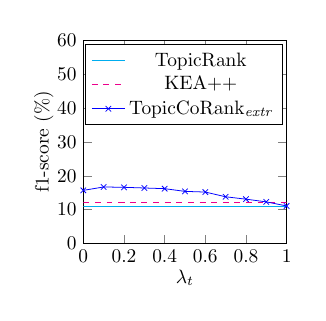
\begin{tikzpicture}[scale=.7]
                    \pgfkeys{/pgf/number format/.cd, fixed}
                    \begin{axis}[x=0.304152\linewidth,
                                 xtick={0, 0.2, 0.4, ..., 1},
                                 xmin=0,
                                 xmax=1,
                                 xlabel=$\lambda_t$,
                                 x label style={yshift=.34em},
                                 y=0.0050692\linewidth,
                                 ytick={0, 10, 20, ..., 100},
                                 ymin=0,
                                 ymax=60,
                                 ylabel=f1-score (\%),
                                 y label style={yshift=-.5em}]
                        \addplot[cyan] coordinates{
                            (0.0, 11)
                            (0.2, 11)
                            (0.3, 11)
                            (0.4, 11)
                            (0.5, 11)
                            (0.6, 11)
                            (0.7, 11)
                            (0.8, 11)
                            (0.9, 11)
                            (1.0, 11)
                        };
                        \addplot[magenta, dashed] coordinates{
                            (0.0, 12)
                            (0.2, 12)
                            (0.3, 12)
                            (0.4, 12)
                            (0.5, 12)
                            (0.6, 12)
                            (0.7, 12)
                            (0.8, 12)
                            (0.9, 12)
                            (1.0, 12)
                        };
                        \addplot[blue, mark=x] coordinates{
                            (0.0, 15.7)
                            (0.1, 16.7)
                            (0.2, 16.6)
                            (0.3, 16.4)
                            (0.4, 16.2)
                            (0.5, 15.4)
                            (0.6, 15.2)
                            (0.7, 13.8)
                            (0.8, 13.1)
                            (0.9, 12.3)
                            (1.0, 11.1)
                        };
                        \legend{TopicRank, KEA++, TopicCoRank$_\textit{extr}$};
                    \end{axis}
                \end{tikzpicture}
            }
            \subfigure[Information Science]{
                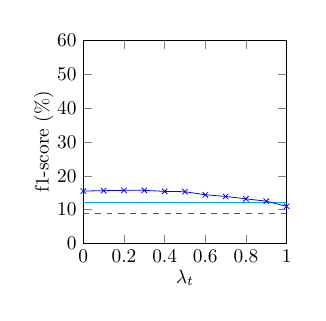
\begin{tikzpicture}[scale=.7]
                    \pgfkeys{/pgf/number format/.cd, fixed}
                    \begin{axis}[x=0.304152\linewidth,
                                 xtick={0, 0.2, 0.4, ..., 1},
                                 xmin=0,
                                 xmax=1,
                                 xlabel=$\lambda_t$,
                                 x label style={yshift=.34em},
                                 y=0.0050692\linewidth,
                                 ytick={0, 10, 20, ..., 100},
                                 ymin=0,
                                 ymax=60,
                                 ylabel=f1-score (\%),
                                 y label style={yshift=-.5em}]
                        \addplot[cyan] coordinates{
                            (0.0, 12)
                            (0.2, 12)
                            (0.3, 12)
                            (0.4, 12)
                            (0.5, 12)
                            (0.6, 12)
                            (0.7, 12)
                            (0.8, 12)
                            (0.9, 12)
                            (1.0, 12)
                        };
                        \addplot[magenta, dashed] coordinates{
                            (0.0, 9)
                            (0.2, 9)
                            (0.3, 9)
                            (0.4, 9)
                            (0.5, 9)
                            (0.6, 9)
                            (0.7, 9)
                            (0.8, 9)
                            (0.9, 9)
                            (1.0, 9)
                        };
                        \addplot[blue, mark=x] coordinates{
                            (0.0, 15.5)
                            (0.1, 15.6)
                            (0.2, 15.7)
                            (0.3, 15.7)
                            (0.4, 15.4)
                            (0.5, 15.3)
                            (0.6, 14.4)
                            (0.7, 13.9)
                            (0.8, 13.2)
                            (0.9, 12.5)
                            (1.0, 11.0)
                        };
                    \end{axis}
                \end{tikzpicture}
            }
            \subfigure[Archaeology]{
                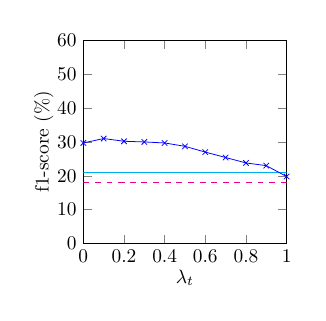
\begin{tikzpicture}[scale=.7]
                    \pgfkeys{/pgf/number format/.cd, fixed}
                    \begin{axis}[x=0.304152\linewidth,
                                 xtick={0, 0.2, 0.4, ..., 1},
                                 xmin=0,
                                 xmax=1,
                                 xlabel=$\lambda_t$,
                                 x label style={yshift=.34em},
                                 y=0.0050692\linewidth,
                                 ytick={0, 10, 20, ..., 100},
                                 ymin=0,
                                 ymax=60,
                                 ylabel=f1-score (\%),
                                 y label style={yshift=-.5em},
                                 legend style={font=\footnotesize}]
                        \addplot[cyan] coordinates{
                            (0.0, 21)
                            (0.2, 21)
                            (0.3, 21)
                            (0.4, 21)
                            (0.5, 21)
                            (0.6, 21)
                            (0.7, 21)
                            (0.8, 21)
                            (0.9, 21)
                            (1.0, 21)
                        };
                        \addplot[magenta, dashed] coordinates{
                            (0.0, 18)
                            (0.2, 18)
                            (0.3, 18)
                            (0.4, 18)
                            (0.5, 18)
                            (0.6, 18)
                            (0.7, 18)
                            (0.8, 18)
                            (0.9, 18)
                            (1.0, 18)
                        };
                        \addplot[blue, mark=x] coordinates{
                            (0.0, 29.7)
                            (0.1, 31.0)
                            (0.2, 30.2)
                            (0.3, 30.0)
                            (0.4, 29.7)
                            (0.5, 28.7)
                            (0.6, 27.0)
                            (0.7, 25.4)
                            (0.8, 23.8)
                            (0.9, 23.0)
                            (1.0, 19.8)
                        };
                    \end{axis}
                \end{tikzpicture}
            }
            \caption{
                Behavior of TopicCoRank$_\textit{extr}$ depending on $\lambda_t$ ($\lambda_k = 0.5$)
                \label{fig:lambda_t_variation}
            }
        \end{figure}
        
        %\begin{figure}[t]
        %    \centering
        %    \subfigure[TopicCoRank$_\textit{extr}$~($\lambda_k$~$=$~$0.5$)\label{subfig:topiccorank_extr}]{
        %        \begin{tikzpicture}[scale=.6]
        %            \pgfkeys{/pgf/number format/.cd, fixed}
        %            \begin{axis}[x=0.5\linewidth,
        %                         xtick={0, 0.2, ..., 1.0},
        %                         xmin=0.0,
        %                         xmax=1.0,
        %                         xlabel=$\lambda_t$,
        %                         x label style={yshift=.34em},
        %                         y=0.0083375\textheight,
        %                         ytick={0, 4, ..., 100},
        %                         ymin=4,
        %                         ymax=44,
        %                         ylabel=f1-score (\%),
        %                         y label style={yshift=-1.1em}]
        %                \addplot[cyan, mark=+] coordinates{
        %                    (0.0, 15.7)
        %                    (0.1, 16.7)
        %                    (0.2, 16.6)
        %                    (0.3, 16.4)
        %                    (0.4, 16.2)
        %                    (0.5, 15.4)
        %                    (0.6, 15.2)
        %                    (0.7, 13.8)
        %                    (0.8, 13.1)
        %                    (0.9, 12.3)
        %                    (1.0, 11.1)
        %                };
        %                \addplot[magenta, mark=o] coordinates{
        %                    (0.0, 15.5)
        %                    (0.1, 15.6)
        %                    (0.2, 15.7)
        %                    (0.3, 15.7)
        %                    (0.4, 15.4)
        %                    (0.5, 15.3)
        %                    (0.6, 14.4)
        %                    (0.7, 13.9)
        %                    (0.8, 13.2)
        %                    (0.9, 12.5)
        %                    (1.0, 11.0)
        %                };
        %                \addplot[black!75, mark=x] coordinates{
        %                    (0.0, 29.7)
        %                    (0.1, 31.0)
        %                    (0.2, 30.2)
        %                    (0.3, 30.0)
        %                    (0.4, 29.7)
        %                    (0.5, 28.7)
        %                    (0.6, 27.0)
        %                    (0.7, 25.4)
        %                    (0.8, 23.8)
        %                    (0.9, 23.0)
        %                    (1.0, 19.8)
        %                };
        %                \legend{Linguistics, Information Science, Archaeology};
        %            \end{axis}
        %        \end{tikzpicture}
        %    }
        %    \hspace{1em}
        %    \subfigure[TopicCoRank$_\textit{assign}$~($\lambda_t$~$=$~$0.1$)\label{subfig:topiccorank_assign}]{
        %        \begin{tikzpicture}[scale=.6]
        %            \pgfkeys{/pgf/number format/.cd, fixed}
        %            \begin{axis}[x=0.5\linewidth,
        %                         xtick={0, 0.2, ..., 1.0},
        %                         xmin=0.0,
        %                         xmax=1.0,
        %                         xlabel=$\lambda_k$,
        %                         x label style={yshift=.34em},
        %                         y=0.0083375\textheight,
        %                         ytick={0, 4, ..., 100},
        %                         ymin=4,
        %                         ymax=44,
        %                         ylabel=f1-score (\%),
        %                         y label style={yshift=-1.1em}]
        %                \addplot[cyan, mark=+] coordinates{
        %                    (0.0, 21.0)
        %                    (0.2, 24.7)
        %                    (0.3, 25.4)
        %                    (0.4, 25.7)
        %                    (0.5, 27.2)
        %                    (0.6, 24.9)
        %                    (0.7, 18.0)
        %                    (0.8, 17.0)
        %                    (0.9, 16.6)
        %                    (1.0, 16.4)
        %                };
        %                \addplot[magenta, mark=o] coordinates{
        %                    (0.0, 17.6)
        %                    (0.1, 18.4)
        %                    (0.2, 18.3)
        %                    (0.3, 18.6)
        %                    (0.4, 19.2)
        %                    (0.5, 19.5)
        %                    (0.6, 19.4)
        %                    (0.7, 11.8)
        %                    (0.8, 8.7)
        %                    (0.9, 7.7)
        %                    (1.0, 7.5)
        %                };
        %                \addplot[black!75, mark=x] coordinates{
        %                    (0.0, 31.4)
        %                    (0.1, 35.1)
        %                    (0.2, 35.5)
        %                    (0.3, 35.6)
        %                    (0.4, 36.7)
        %                    (0.5, 39.0)
        %                    (0.6, 33.0)
        %                    (0.7, 23.5)
        %                    (0.8, 21.4)
        %                    (0.9, 20.4)
        %                    (1.0, 20.4)
        %                };
        %            \end{axis}
        %        \end{tikzpicture}
        %    }
        %    \caption{
        %        Behavior of TopicCoRank$_\textit{extr}$ and TopicCoRank$_\textit{assign}$ according to $\lambda_t$ and $\lambda_k$, %respectively
        %        \label{fig:lambda_variation}
        %    }
        %\end{figure}
        
        Fig.~\ref{fig:lambda_k_variation} shows the behavior of TopicCo\-Rank$_\textit{assign}$ when $\lambda_k$ varies from 0 to 1.
        When $\lambda_k = 0$, only the document influences the ranking of the controlled keyphrases.
        As for TopicCoRank$_\textit{extr}$ when $\lambda_t = 0$, TopicCoRank$_\textit{assign}$ is slightly similar to KEA++ when $\lambda_k = 0$.
        When $\lambda_k = 1$, TopicCoRank$_\textit{assign}$ always outputs the same keyphrases: the ones that are the most important in the domain.
        %This configuration achieves the lowest performance, which is understandable, yet still competitive with the baselines. % because of general keyphrases manually assigned to a large amount of documents.
        The first half of the curve increases, showing that the relations between the controlled keyphrases have a positive influence on the ranking of the controlled keyphrases.
        Conversely, the second half of the curve decreases.
        Thus, the sole domain is not sufficient for keyphrase annotation.
        
        \begin{figure}[htb!]
            \centering
            \subfigure[Linguistics]{
                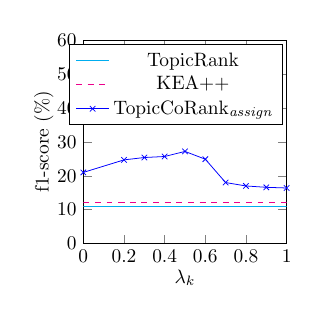
\begin{tikzpicture}[scale=.7]
                    \pgfkeys{/pgf/number format/.cd, fixed}
                    \begin{axis}[x=0.304152\linewidth,
                                 xtick={0, 0.2, 0.4, ..., 1},
                                 xmin=0,
                                 xmax=1,
                                 xlabel=$\lambda_k$,
                                 x label style={yshift=.34em},
                                 y=0.0050692\linewidth,
                                 ytick={0, 10, 20, ..., 100},
                                 ymin=0,
                                 ymax=60,
                                 ylabel=f1-score (\%),
                                 y label style={yshift=-.5em}]
                        \addplot[cyan] coordinates{
                            (0.0, 11)
                            (0.2, 11)
                            (0.3, 11)
                            (0.4, 11)
                            (0.5, 11)
                            (0.6, 11)
                            (0.7, 11)
                            (0.8, 11)
                            (0.9, 11)
                            (1.0, 11)
                        };
                        \addplot[magenta, dashed] coordinates{
                            (0.0, 12)
                            (0.2, 12)
                            (0.3, 12)
                            (0.4, 12)
                            (0.5, 12)
                            (0.6, 12)
                            (0.7, 12)
                            (0.8, 12)
                            (0.9, 12)
                            (1.0, 12)
                        };
                        \addplot[blue, mark=x] coordinates{
                            (0.0, 21.0)
                            (0.2, 24.7)
                            (0.3, 25.4)
                            (0.4, 25.7)
                            (0.5, 27.2)
                            (0.6, 24.9)
                            (0.7, 18.0)
                            (0.8, 17.0)
                            (0.9, 16.6)
                            (1.0, 16.4)
                        };
                        \legend{TopicRank, KEA++, TopicCoRank$_\textit{assign}$};
                    \end{axis}
                \end{tikzpicture}
            }
            \subfigure[Information Science]{
                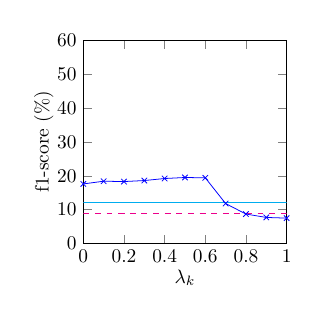
\begin{tikzpicture}[scale=.7]
                    \pgfkeys{/pgf/number format/.cd, fixed}
                    \begin{axis}[x=0.304152\linewidth,
                                 xtick={0, 0.2, 0.4, ..., 1},
                                 xmin=0,
                                 xmax=1,
                                 xlabel=$\lambda_k$,
                                 x label style={yshift=.34em},
                                 y=0.0050692\linewidth,
                                 ytick={0, 10, 20, ..., 100},
                                 ymin=0,
                                 ymax=60,
                                 ylabel=f1-score (\%),
                                 y label style={yshift=-.5em}]
                        \addplot[cyan] coordinates{
                            (0.0, 12)
                            (0.2, 12)
                            (0.3, 12)
                            (0.4, 12)
                            (0.5, 12)
                            (0.6, 12)
                            (0.7, 12)
                            (0.8, 12)
                            (0.9, 12)
                            (1.0, 12)
                        };
                        \addplot[magenta, dashed] coordinates{
                            (0.0, 9)
                            (0.2, 9)
                            (0.3, 9)
                            (0.4, 9)
                            (0.5, 9)
                            (0.6, 9)
                            (0.7, 9)
                            (0.8, 9)
                            (0.9, 9)
                            (1.0, 9)
                        };
                        \addplot[blue, mark=x] coordinates{
                            (0.0, 17.6)
                            (0.1, 18.4)
                            (0.2, 18.3)
                            (0.3, 18.6)
                            (0.4, 19.2)
                            (0.5, 19.5)
                            (0.6, 19.4)
                            (0.7, 11.8)
                            (0.8, 8.7)
                            (0.9, 7.7)
                            (1.0, 7.5)
                        };
                    \end{axis}
                \end{tikzpicture}
            }
            \subfigure[Archaeology]{
                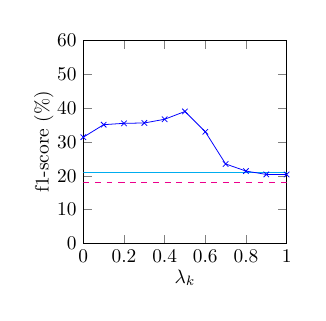
\begin{tikzpicture}[scale=.7]
                    \pgfkeys{/pgf/number format/.cd, fixed}
                    \begin{axis}[x=0.304152\linewidth,
                                 xtick={0, 0.2, 0.4, ..., 1},
                                 xmin=0,
                                 xmax=1,
                                 xlabel=$\lambda_k$,
                                 x label style={yshift=.34em},
                                 y=0.0050692\linewidth,
                                 ytick={0, 10, 20, ..., 100},
                                 ymin=0,
                                 ymax=60,
                                 ylabel=f1-score (\%),
                                 y label style={yshift=-.5em},
                                 legend style={font=\footnotesize}]
                        \addplot[cyan] coordinates{
                            (0.0, 21)
                            (0.2, 21)
                            (0.3, 21)
                            (0.4, 21)
                            (0.5, 21)
                            (0.6, 21)
                            (0.7, 21)
                            (0.8, 21)
                            (0.9, 21)
                            (1.0, 21)
                        };
                        \addplot[magenta, dashed] coordinates{
                            (0.0, 18)
                            (0.2, 18)
                            (0.3, 18)
                            (0.4, 18)
                            (0.5, 18)
                            (0.6, 18)
                            (0.7, 18)
                            (0.8, 18)
                            (0.9, 18)
                            (1.0, 18)
                        };
                        \addplot[blue, mark=x] coordinates{
                            (0.0, 31.4)
                            (0.1, 35.1)
                            (0.2, 35.5)
                            (0.3, 35.6)
                            (0.4, 36.7)
                            (0.5, 39.0)
                            (0.6, 33.0)
                            (0.7, 23.5)
                            (0.8, 21.4)
                            (0.9, 20.4)
                            (1.0, 20.4)
                        };
                    \end{axis}
                \end{tikzpicture}
            }
            \caption{
                Behavior of TopicCoRank$_\textit{assign}$ depending on $\lambda_k$ ($\lambda_t = 0.1$)
                \label{fig:lambda_k_variation}
            }
        \end{figure}

  \subsection{Qualitative example}
\label{subsec:qualitative_example}
    \REVIEWOK{We need the authors to explain clearly and deeply why TopicCoRank can outperform TopicRank}
    To show the benefit of TopicCoRank, we compare it to TopicRank on one of our bibliographic records in Linguistics (see Figure~\ref{fig:example}).
    Over the nine reference keyphrases, TopicRank successfully identifies two of the reference keyphrases: ``lexical semantics'' and ``semantic variation''. TopicCoRank successfully identifies seven of them: ``lexical semantics'', ``verb'', ``semantic variation'', ``French'', ``syntax'', ``semantic interpretation'' and ``distributional analysis''.
    
    \begin{figure}
      \centering
      \framebox[\linewidth]{
        \parbox{.99\linewidth}{\footnotesize
          \textbf{\textit{Toucher : le tango des sens. Problèmes de sémantique lexicale} (The French verb 'toucher': the tango of senses. A problem of lexical)}\\
    
          \textit{A partir d'une hypothèse sur la sémantique de l'unité lexicale 'toucher' formulée en termes de forme schématique, cette étude vise à rendre compte de la variation sémantique manifestée par les emplois de ce verbe dans la construction transitive directe 'C0 toucher C1'. Notre étude cherche donc à articuler variation sémantique et invariance fonctionnelle. Cet article concerne essentiellement le mode de variation co-textuelle : en conséquence, elle ne constitue qu'une première étape dans la compréhension de la construction des valeurs référentielles que permet 'toucher'. Une étude minutieuse de nombreux exemples nous a permis de dégager des constantes impératives sous la forme des 4 notions suivantes : sous-détermination sémantique, contact, anormalité, et contingence. Nous avons tenté de montrer comment ces notions interprétatives sont directement dérivables de la forme schématique proposée.}\\
    
          \textbf{Keyphrases~}:
            \textit{Français} (French); \textit{modélisation} (modelling); \textit{analyse distributionnelle} (distributional analysis); \textit{interprétation sémantique} (semantic interpretation); \textit{variation sémantique} (semantic variation); \textit{transitif} (transitive); \textit{verbe} (verb); \textit{syntaxe} (syntax) and \textit{sémantique lexicale} (lexical semantics).
        }
      }
      \caption{Example of a bibliographic record in Linguistics (\url{http://cat.inist.fr/?aModele=afficheN&cpsidt=16471543})\label{fig:example}}
    \end{figure}

    TopicCoRank mostly outperforms TopicRank because it finds key\-phrases that do not occur within the document: ``French'', ``syntax'', ``semantic interpretation'', and ``distributional analysis''.
    Some keyphrases, such as ``French'', are frequently assigned because they are part of most of the bibliographic records of our dataset\footnote{Yet, TopicCoRank does not assign ``French'' to every bibliographic records.} (48.9\% of the Linguistics records contain ``French'' as a keyphrase);
    Other keyphrases, such as ``semantic interpretation'', are assigned thanks to their strong connection with controlled keyphrases occurring in the abstract (e.g.~``lexical semantics'').

    Interestingly, the performance of TopicCoRank is not only better thanks to the assignment.
    For instance, we observe keyphrases, such as ``verb'', that emerge from topics connected to other topics that distribute importance from controlled keyphrases (e.g.~``semantic variation'').

  \section{Conclusion et perspectives}
\label{sec:conclusion_et_perspectives}
  Dans ce travail, nous proposons une méthode à base de graphe pour l'extraction
  non supervisée de termes-clés. Cette méthode groupe les termes-clés candidats
  en sujets, détermine quels sont ceux les plus importants, puis extrait le
  terme-clé candidat qui représente le mieux chacun des sujets les plus
  importants. Cette nouvelle méthode offre plusieurs avantages vis-à-vis des
  précédentes à base de graphe. Le groupement des termes-clés potentiels en
  sujets distincts permet de rassembler des indices utiles auparavant éparpillés
  et le choix d'un seul terme-clé pour représenter un sujet important permet
  d'extraire un ensemble de termes-clés non redondants ( pour $k$ termes-clés
  extraits, exactement $k$ sujets sont couverts). Enfin, le graphe est complet
  et ne requiert plus le paramétrage d'une fenêtre de cooccurrences,
  contrairement aux autres méthodes à base de graphe.

  Les bons résultats de notre méthode montrent la pertinence d'un groupement en
  sujets des candidats pour ensuite les ordonner. Les expériences
  supplémentaires montrent aussi qu'il est encore possible d'améliorer notre
  méthode en proposant une nouvelle stratégie de sélection du terme-clé candidat
  le plus représentatif d'un sujet (pour un gain maximum allant de 4,2 à 15
  points de f-score).

  Nous avons aussi effectué une analyse d'erreurs à partir de laquelle trois
  perspectives de travaux futurs émergent~:

  Nous avons pour objectif d'améliorer la sélection des termes-clés candidats.
  Aussi, des méthodes empruntées à d'autres domaines du TAL peuvent être
  appliquées. Il semble, par exemple, pertinent d'évaluer l'apport des méthodes
  d'extraction terminologiques~\cite{castellvi2001automatictermdetection} pour
  la sélection des termes-clés candidats.
  
  Nous envisageons également d'améliorer le groupement en sujets,
  car celui-ci est très naïf et ne tient compte ni de la synonymie, ni de
  l'ambiguïté des mots. De plus, l'usage du
  radical~\cite{porter1980suffixstripping} des mots n'est pas sans introduire du
  bruit lié à certains faux positifs (p.~ex. \og{}\underline{empir}e\fg{} et
  \og{}\underline{empir}ique\fg{}). L'ajout de connaissances concernant les
  synonymes permettrait de créer des sujets plus complets et une étape de
  désambiguïsation éviterait un groupement systématique des termes-clés
  candidats ayant un ou plusieurs mots en commun. Nous envisageons aussi de
  remplacer la racinisation de \newcite{porter1980suffixstripping} par une
  méthode de lemmatisation. D'un point de vue plus technique, il faudrait
  explorer différentes méthodes de groupement, dont le groupement spectral
  (\textit{spectral clustering}) qui, dans d'autres travaux portant sur
  l'extraction automatique de termes-clés~\cite{liu2009keycluster}, montre de
  meilleures performances que le groupement hiérarchique agglomératif.

  Enfin, une étude détaillée des caractéristiques des termes-clés pourrait
  orienter notre travail vers des critères plus efficaces pour la définition
  d'une stratégie \og{}optimale\fg{} de sélection du terme-clé le plus
  représentatif d'un sujet. Un apprentissage supervisé à partir de certains
  critères est aussi envisagé, au même titre que l'usage de méthodes
  d'optimisation, telles que celle utilisée par
  \newcite{ding2011binaryintegerprogramming} dans leur méthode d'extraction
  automatique de termes-clés.



  \bibliographystyle{plainnat.min}
  \renewcommand\bibname{References}
  \bibliography{biblio}
\end{document}
